% Created 2022-05-19 Thu 14:47
% Intended LaTeX compiler: pdflatex
\documentclass{article}
\usepackage[utf8]{inputenc}
\usepackage[T1]{fontenc}
\usepackage{graphicx}
\usepackage{longtable}
\usepackage{wrapfig}
\usepackage{rotating}
\usepackage[normalem]{ulem}
\usepackage{amsmath}
\usepackage{amssymb}
\usepackage{capt-of}
\usepackage{hyperref}
\usepackage[cachedir=/tmp/minted]{minted}
\usepackage{color}
\usepackage{tikz}
\usepackage{fancyvrb}
\usepackage[a4paper]{anysize}
\usepackage{minted}
\usepackage{xparse}
\newminted{c}{tabsize=4,obeytabs,autogobble,highlightcolor=gray!20}
\newenvironment{env}{\VerbatimEnvironment\begin{ccode}}{\end{ccode}}
\newmintinline{c}{}
\newmintedfile{c}{tabsize=4,obeytabs,linenos,frame=single,highlightcolor=gray!50}
\setcounter{secnumdepth}{4}
\author{Niclas Borlin (\texttt{niclas.borlin@cs.umu.se})}
\date{2022-05-19}
\title{5DV149 LP4 --- Assignment 4\\\medskip
\large Graphs\\
Submission v1.0}
\begin{document}

\maketitle
\clearpage \tableofcontents \clearpage\addtocounter{section}{-1}
\section{Version history}
\label{sec:history}
\begin{description}
\item[{v1.0 2022-05-19}] First submission.\footnote{If this is a resubmission, include a list of changes with
respect to the previous submission.}
\end{description}

\section{Introduction}
\label{sec:intro}
The target audience is someone with basic understanding in Computing
Science, but not specifically graphs nor the application, e.g., a
future colleague at your work who did not take part in this particular
project. Describe the application and how it connects to graphs. You
may include a figure, e.g. as in figures \ref{fig:graph1} and \ref{fig:graph2}.

\begin{figure}[tbp]
\centering
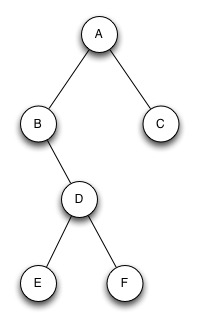
\includegraphics[width=0.2\hsize]{graph1.png}
\caption{\label{fig:graph1}Graph illustration corresponding to the file \texttt{airmap1.map}, png version.}
\end{figure}

\begin{figure}
  \begin{center}
    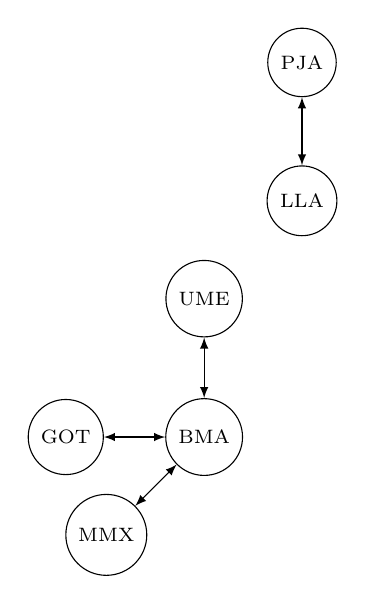
\begin{tikzpicture}[node distance=5em,font=\scriptsize]
      \node[draw,circle] (ume) { UME };
      \node[draw,circle,below of=ume] (bma) { BMA };
      \node[draw,circle,below left of=bma] (mmx) { MMX };
      \node[draw,circle,left of=bma] (got) { GOT };
      \node[draw,circle,above right of=ume] (lla) { LLA };
      \node[draw,circle,above of=lla] (pja) { PJA };
      \draw[latex-latex] (ume) -- (bma);
      \draw[latex-latex] (mmx) -- (bma);
      \draw[latex-latex] (got) -- (bma);
      \draw[latex-latex] (lla) -- (pja);
    \end{tikzpicture}
  \end{center}
\caption{\label{fig:graph2}Graph illustration corresponding to the file \texttt{airmap1.map}, tikz version.}
\end{figure}

\section{User guide}
\label{sec:user_guide}
\subsection{Compilation}
\label{sec:compilation}
Describe exactly how the reader might compile the code, assuming
he/she has access to the source code, e.g.
\phantomsection
\label{example:compile}
\begin{verbatim}
gcc -o is_connected -std=c99 -Wall -I .../path/to/include is_connected.c graph.c
  .../path/to/other/files.c
\end{verbatim}
\subsection{File format}
\label{sec:file_format}
Describe the file format, including an example, e.g. (NOTE: you MUST change this example!)
\begin{verbatim}
# This is a text file
2
UME BMA # Umea-Bromma
BMA UME # Bromma-Umea
\end{verbatim}
\subsection{Test runs}
\label{sec:test_run}
Describe a complete test run, i.e., how the program is started, input
and output. Screen dumps can be useful here, but be sure to trim them
to the terminal window where the program is run.
\section{System description}
\label{sec:system_description}
\subsection{Data structures}
\label{sec:org6e002c6}
\subsubsection{Graph}
\label{sec:graph}
The graph data structure is central to this assignment. Describe how
you have designed and implemented the data structure. What information
is stored and where? If you use a \texttt{struct}, you should probably
describe it and its fields. How is the allocate/deallocate
responsibility handled. What help data structures have you used? How
have you defined equality between nodes? How do you handle (avoid?)
node duplicate in the graph?

Describe each function in the interface to the data type \texttt{Graph}. Each
implemented function should be described in some detail, e.g., input,
output, actions and any side effects. The interface should be
organised to be easy to read, e.g., in a table or a bullet list. It is
ok to include the function declaration, e.g.,\footnote{If you use latex and minted for this kind of color-coding
of source code you must probably need to compile the .tex file with
\texttt{pdflatex -shell-escape file.tex}.}
\begin{ccode}
graph *graph_insert_edge(graph *g, node *n1, node *n2);
\end{ccode}
but in the text you should refer to \emph{the graph \texttt{g}}, \emph{the node \texttt{n1}},
etc. Never use \texttt{*} in the text. Instead, if it is necessary, write
''pointer to\ldots{}''.

You may group and the unimplemented functions separately. The
unimplemented function do not need to be described nor commented, only
listed.

\subsubsection{Graph \#2}
\label{sec:graph2}
If you have implemented two different graphs, describe the second
implementation here.

\subsubsection{Other data structures}
\label{sec:other_data_structures}
For each data type from the code base that you have used, e.g.,
\texttt{queue}, describe it in a separate subsection. In each section,
describe the datatype briefly in one or a few sentences and then list
all functions in the user interface. Only make references to
\emph{published} information about the data type. That includes what is
known from the header files but not the source.

\subsection{Algorithms}
\label{sec:algorithms}
All algorithms must be described in \emph{psedocode}. You may use text to
summarize the algorithm, but each step must be in some form of
bulleted or enumerated list. Remember to use variable names, etc., to
make the algorithm more specific, e.g., ''the current node \(n\)'', etc.
\subsubsection{Parsing the text file and constructing the graph}
\label{sec:parse}
Describe your algorithm for parsing the text file and constructing the
graph. Depending on your implementation, this may be one algorithm or
two separate ones. You do not have to describe the parsing of each
line in detail.
\subsubsection{\texttt{find\_path}}
\label{sec:find_path}
Describe your version of the breadth-first-algorithm that you have
implemented in \texttt{find\_path}.
\section{Reflections}
\label{sec:orgd37f281}
\subsection{Work distribution}
\label{sec:org66520d9}
If you worked in groups, how has the work been distributed. How have
you made sure that everyone understands each part, including parts
that have been the resposibility of others?
\subsection{Reflections}
\label{sec:org2c6da4f}
Reflect on the assignment! Did you find anything fun, challenging,
surprising, frustrating, rewarding, etc. If you submit for a group,
you may write one reflection for each group member, or one for the whole group.

\subsection{Future work (optional)}
\label{sec:org2c448d8}

Did you think of anything interesting to try that you did not have
time to include? If yes, this is the place to present it.

\clearpage\appendix


\section{Useful \LaTeX{} examples}
\label{app:useful-latex-examples}
Stuff that may be important to some readers, but not all, may be
deferred to an appendix. The same is true for lengthy material that
would disrupt the flow of the document if placed immediately where it
is first referenced. Examples include code listings, file formats,
standards, complete tables of all experiments, etc.

\subsection{Figures}
\label{app:figures}
Figure \ref{fig:image} shows an example of a figure. Exactly \emph{where} (at top
or bottom of a page, on a separate page, or ''here'' in the text) to
put figures/tables is a matter of style. The author of this document
is of the opinion that ''here'' should be avoided at all cost. It
might seem advantageous to have the figure close to the text that
describes it. However, the figure/table should be as self-contained as
possible. In general, it should be possible to read and understand the
body text \emph{without} having to look at the figure. Thus, if you are
forced to write the body text and present the figure such that they
will work independently, your report and writing style will benefit.

As the placement of figures and other floats in \LaTeX{} may shift due to
changes in text, you are encouraged to leave the fine-tuning of image
placement \textbf{until your document is complete}.

\begin{figure}[tbp]
\centering
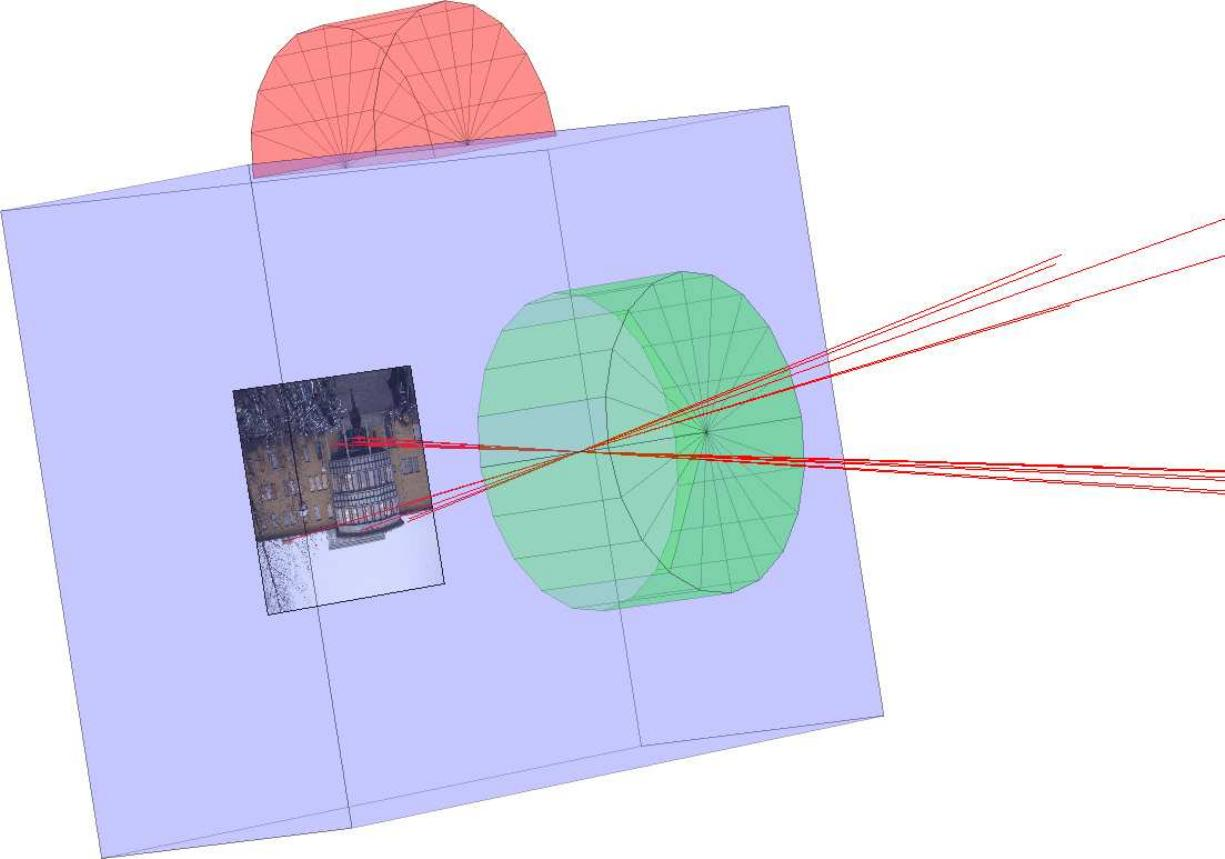
\includegraphics[width=0.7\hsize]{./camwithimage8.jpg}
\caption{\label{fig:image}A figure/image caption should provide sufficient information to make the figure/image as self-explanatory as possible. The caption should be placed under the figure. The latex source shows how to include an image file into a latex document.}
\end{figure}

\subsection{Tables}
\label{app:tables}
Tables are often used to present tabulated (no sh*t, sherlock?) data
about the experiment setup, test data, etc., or with results of the
experiments. In the former case, the body text would typically
describe what is common with the data sets and then refer to a table
with detailed information. In the latter case, do not discuss the
structure of the table in the body text! That would just confuse the
reader. Such information belongs to the caption. In general, do not
refer to the table such that the reader cannot continue without
inspecting the table. Instead, summarize enough of the content of the
table to allow the reader to continue to the next paragraph.

Data that can better be summarized in the body text should so appear,
e.g., ''The execution time for experiment x was below 2ms. The other
execution times are given in Table x.''

In all cases, consider the number of significant digits! Do not put a
gazillion decimals in your tables just because your code spits it out!
Make the table as easy to read as possible. An example of a stub of a
results table is given in Table \ref{tab:time-table}.

\begin{table}[tbp]
\caption{\label{tab:time-table}A table caption should provide information that helps the reader to understand what data is in the table. Some additional information, e.g., units can also be part of the caption. A table caption should be placed above the table proper. Use as few borders in the table as possible! For instance, adding left and right borders to the table below would make it harder to read.}
\centering
\begin{tabular}{l|l}
\textbf{Table type} & Lookup speed (ms)\\
\hline
MTFTable & x\\
Arraytable & y\\
DListTable & z\\
\end{tabular}
\end{table}
\end{document}